\chapter{Evaluation}\label{ch:Evaluation}
In this chapter, the produced artefact will be evaluated against its original requirements.
In addition, the development process itself will be reflected upon to identify where issues arose 
and could have been prevented.

\section{Methodology}\label{sec:DeepEval}
% Within Section \ref{sec:Requirements}, the functional and non-functional requirements for this project were stated.
% Of these requirements, the chatbot successfully meets all functional requirements, as well as the original aims and 
% objectives stated in \ref{sec:AimsAndObjectives}. However, two non-functional requirements were not met.

% \para One of these requirements was 'The chatbot could allow for voice input and output.' This requirement was not met,
% as it would introduce a significant cost and time investment in trying to integrate this functionality into a Streamlit 
% web app. The other unmet requirement was 'The chatbot could be deployed on an existing messaging service.' This requirement 
% was not met due to time constraints, which is further reflected upon in Section \ref{sec:EvalProcess}. 

\para To properly evaluate the chatbot, it is best to use direct evaluation metrics. While reviewing literature in Section 
\ref{sec:LitReviewLLM}, an evaluation platform known as DeepEval was considered, with the ability to use an LLM as a judge of 
other LLMs \autocite{deepeval_introduction_2024}, known as 'G-Eval', originally created by \textcite{liuGEvalNLGEvaluation2023a}.
This means that the metric is directly programmable using a natural language system prompt as seen with the chatbot itself.

\para 
To evaluate the chatbot, an evaluation dataset of questions and their expected answers was provided, with the chatbot's actual response being
compared to the expected answer which is known to be true (referred to as a 'golden answer'.). It is common practice when using G-Eval to use a 
superior LLM for evaluation than the one that originally generated the answer. Therefore, for G-Eval, gpt-4o was used, making the evaluation process 
the most expensive part of this project's development cycle. 

\subsection{Dataset and evaluation metrics}

\para Table \ref{tab:GoldenDataset} depicts the golden dataset\footnote{BCU's extenuating circumstances policy was updated during the development of the chatbot to where the fourth question's answer is not entirely correct. However, the chatbot is unaware of this, and the objective was to assess the chatbot's performance against its knowledge base sourced in February 2025, so this is not a major issue.} used to evaluate the chatbot's performance, produced by myself after my own in-depth analysis of each policy in the vector store. 

\begin{longtable}{ | p{0.05\linewidth} | p{0.3\linewidth} | p{0.6\linewidth} | }
    \hline
    \cellcolor{blue!25} ID & \cellcolor{blue!25} Question & \cellcolor{blue!25} Expected answer \\
    \hline
    1 & What happens if I submit my assignment 3 days late? &
    If an assignment is submitted 3 days late, your mark will be reduced by 10\%. \\
    \hline
    2 & What happens if I submit my assignment 3 \textbf{minutes} late? &
    If an assignment is submitted 3 minutes late, it is not considered a late submission, and your mark will not be reduced. \\
    \hline 
    3 & What is an EC claim? &
    An Extenuating Circumstances claim can be made by a student if there are circumstances that affect their ability to submit assessments on time, complete assessments to a good standard or attend in-person assessments. \\
    \hline 
    4 & What circumstances will be accepted as extenuating circumstances? &
    Serious short-term illness or injury, worsening of an ongoing illness or disability, symptoms of a harmful infectious disease, death or significant illness of a close family member or friend, unexpected caring responsibilities, significant personal or family crises, witnessing or experiencing a traumatic incident, a crime which has had a substantial impact on you, an accommodation crisis such as eviction.\\
    \hline 
    5 & When must I enrol? & 
    Students must enrol at the start of their programme and enrol for each level by the Friday of week four from the start date of their course unless a Break in Study has been approved. \\
    \hline 
    6 & What is the pass mark for a module? &
    For an undergraduate course, the pass mark is 40\%. On a postgraduate course, it is instead 50\%. \\
    \hline 
    7 & What happens if I fail a module? &
    The first time you fail a module, you can be re-assessed for failed assessments, which is known as a resit. Your grade will be capped at the pass mark. You cannot be reassessed for assessments that you passed. \\ 
    \hline 
    8 & What are the degree classifications? &
    Achieving an average of 70\% or above grants you first-class honours. 60-69\% is an upper second (2:1), 50-59\% is a lower second (2:2), 40-49\% is third-class honours, and anything below 40\% is a fail. \\
    \hline 
    9 & How many BCU students are there? &
    BCU has 31,300 students as of 2022-23. \\ 
    \hline 
    10 & What is BCUSU? &
    The Birmingham City University Student Union represent you as a student, and work together with the university to make change. They can help with various academic topics and offer societies to help people make friends. \\
    \hline
    \caption{The golden dataset for chatbot evaluation.}\label{tab:GoldenDataset}
\end{longtable}

\para The golden dataset was then stored as a nested array of question/answer pairs where for each item in the array, index 0 was the question 
and index 1 was its respective answer. 

\begin{figure}[H]
    \centering
    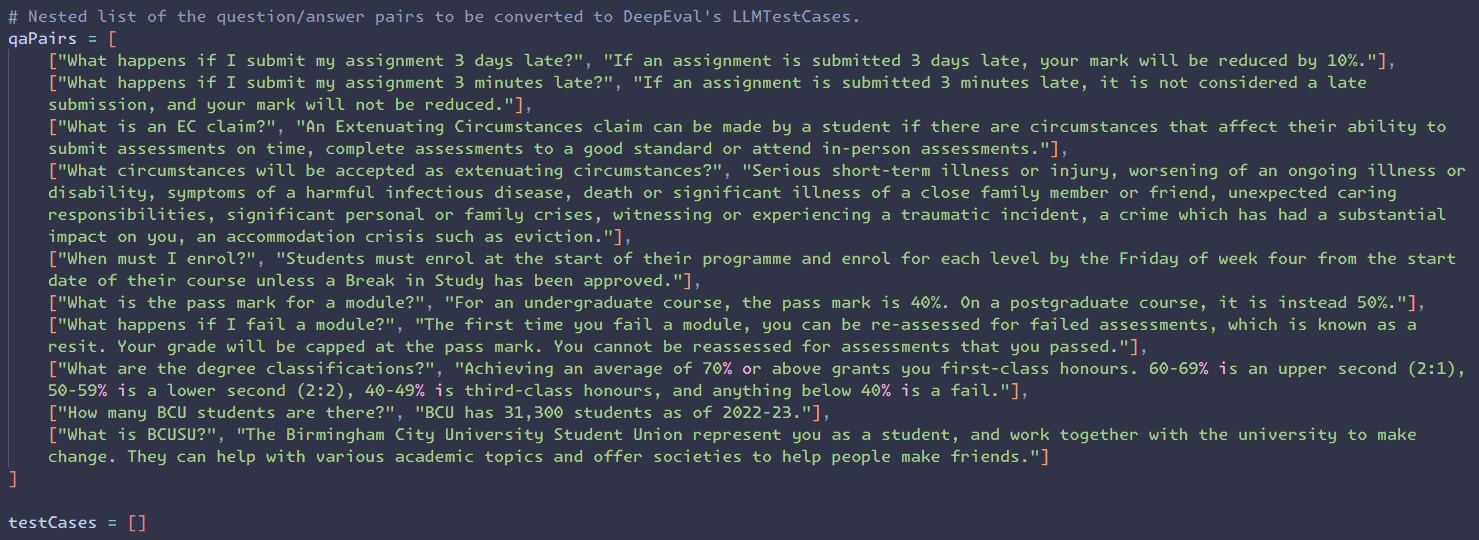
\includegraphics[width=\textwidth]{Evaluation/QAPairs.png}
    \caption{The golden dataset as represented in the evaluation script. \label{fig:GoldenDataset}}
\end{figure}

\noindent To begin testing the chatbot, the 'testChatbot' function was created to invoke the chatbot with 
a sample conversation that is the same as if the Streamlit app had been opened for the first time,
with the only messages being the introductory message and the question from the golden dataset being 
tested.

\begin{figure}[H]
    \centering
    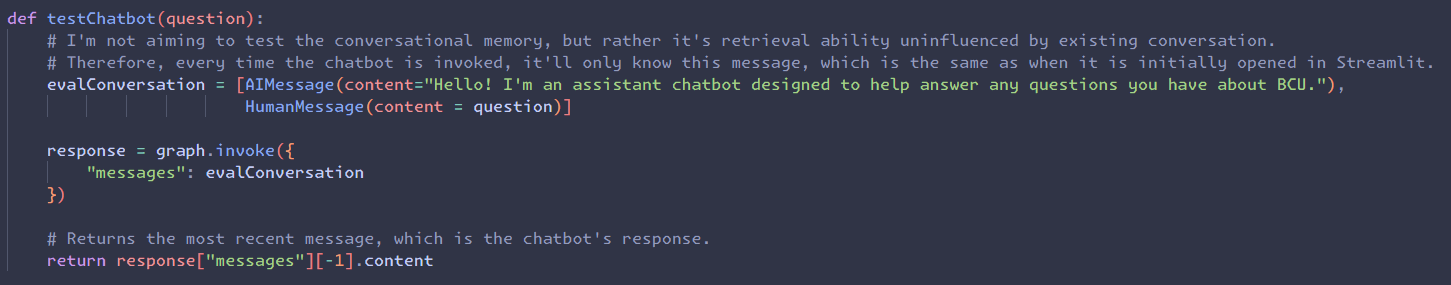
\includegraphics[width=\textwidth]{Evaluation/testChatbot.png}
    \caption{The testChatbot function to invoke the chatbot with a new conversation. \label{fig:testChatbot}}
\end{figure}

\noindent The question/answer pairs were then used to generate DeepEval's own 'LLMTestCase' classes for each item, 
with the input being the question, expected output being the golden answer, and the actual output using the 
testChatbot function to invoke the chatbot.

\begin{figure}[H]
    \centering
    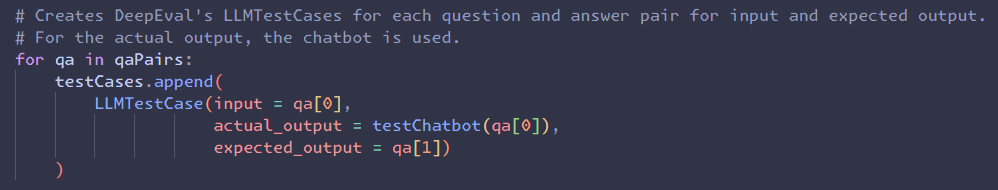
\includegraphics[width=\textwidth]{Evaluation/CreateTestCases.png}
    \caption{Iteratively creating DeepEval LLMTestCases for each question/answer pair. \label{fig:CreateTestCases}}
\end{figure}

\para The test cases were then added into a DeepEval 'EvaluationDataset' for later use. Then, the GEval metric was defined.

\begin{figure}[H]
    \centering
    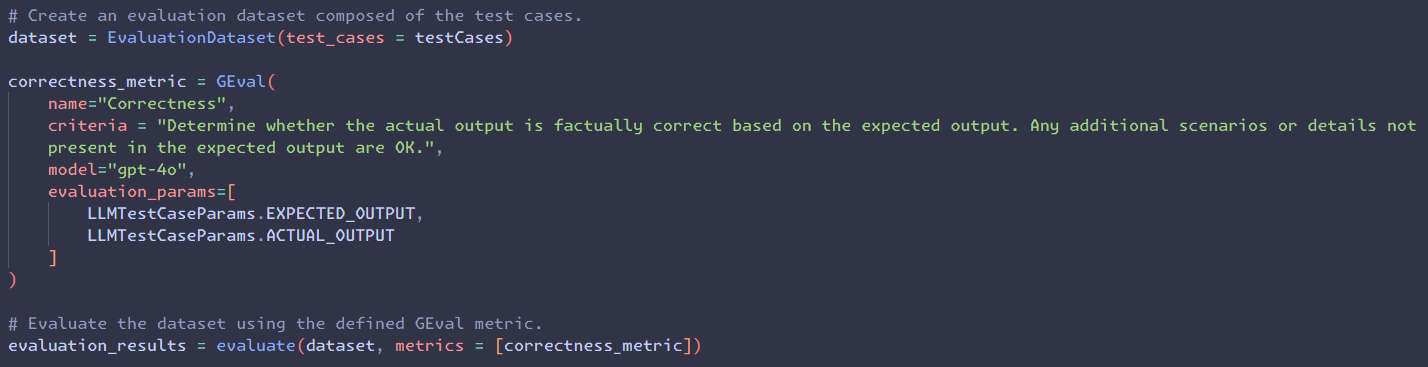
\includegraphics[width=\textwidth]{Evaluation/GEvalMetric.png}
    \caption{Creating the evaluation dataset and GEval metric. \label{fig:GEvalAndDataset}}
\end{figure}

\noindent The criteria field of the GEval metric acts as the system prompt for the gpt-4o model. In the criteria, the LLM is told 
to evaluate the 'correctness' of the actual output by comparing it against the expected output. An additional note was added to ensure 
that the chatbot was not penalised for giving more information than strictly necessary, as GEval would originally fail some test cases 
as the actual output was sometimes more informative than the expected output.

\para Using an LLM for evaluation in this way allows for automated testing to be significantly easier and somewhat more reliable to 
perform, as there is no need for implementations such as word matching. This is because the LLM can automatically infer the semantic 
similarities between the expected answer and the intended answer, known as Semantic Answer Similarity. 

\para Following all of these initial steps, the primary DeepEval 'evaluate' function is called using the created EvaluationDataset
and GEval metric. 

\section{Baseline systems}
Multiple vector stores were created for the chatbot, each using a differing chunk size and overlap. A total of four datasets were 
made, all of which used FAISS as the backend engine and PyPDFLoader to load each PDF prior to chunking. 

\para These vector stores were:
\begin{itemize}
    \item FAISS \begin{itemize}
        \item The original vector store used throughout early development.
        \item Chunk size: 1000
        \item Overlap: 200
    \end{itemize}
    \item FAISS-SmallChunks \begin{itemize}
        \item As suggested by its name, used a lower chunk size and overlap than others.
        \item Chunk size: 500
        \item Overlap: 100 
    \end{itemize}
    \item FAISS-BigChunks \begin{itemize}
        \item Used bigger chunks and overlap than the original vector store.
        \item Chunk size: 1500
        \item Overlap: 300
    \end{itemize}
    \item FAISS-HugeChunks \begin{itemize}
        \item The vector store used in the final product.
        \item Chunk size: 2000
        \item Overlap: 500
    \end{itemize}
\end{itemize}